\documentclass[border=4pt]{standalone}
\usepackage{tikz}
\usetikzlibrary{arrows,arrows.spaced,positioning}
\begin{document}
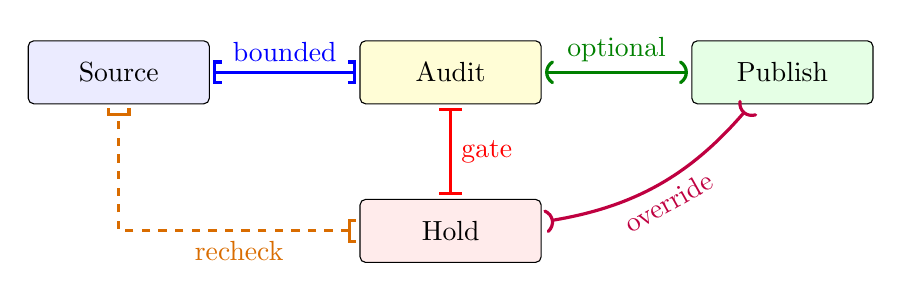
\begin{tikzpicture}[
  node distance=12mm and 19mm,
  stage/.style={draw,rounded corners=2pt,minimum width=23mm,minimum height=8mm,align=center},
  gate/.style={line width=1.15pt}
]
  \node[stage,fill=blue!8] (source) {Source};
  \node[stage,fill=yellow!16,right=of source] (audit) {Audit};
  \node[stage,fill=green!10,right=of audit] (publish) {Publish};
  \node[stage,fill=red!8,below=of audit] (hold) {Hold};

  \draw[gate,blue,arrows={spaced [-spaced ]}]
    (source) -- node[above]{bounded} (audit);
  \draw[gate,green!50!black,arrows={spaced (-spaced )}]
    (audit) -- node[above]{optional} (publish);
  \draw[gate,red,arrows={spaced |-spaced |}]
    (audit) -- node[right]{gate} (hold);
  \draw[gate,dashed,orange!85!black,arrows={spaced ]-spaced [}]
    (hold.west) -| node[pos=.25,below]{recheck} (source.south);
  \draw[gate,purple,arrows={spaced )-spaced (}]
    (hold) to[bend right=20] node[below,sloped]{override} (publish);
\end{tikzpicture}
\end{document}
